\documentclass[12pt]{article}
\usepackage{float}
\usepackage{harvard}
\usepackage[acronym]{glossaries}
\usepackage[automake]{glossaries-extra}
\usepackage{pgfgantt}
\usepackage{graphicx}
\usepackage{array}

\graphicspath{ {./images/} }


\makeglossaries

\newglossaryentry{ictal}
{
        name=latex,
        description={Is a mark up language specially suited for 
scientific documents}
}

\newglossaryentry{preictal}
{
        name=latex,
        description={Is a mark up language specially suited for 
scientific documents}
}

%\acrshort{gcd}
%\acrfull{gcd}
\newacronym{eeg}{EEG}{Electroencephalogram}
\newacronym{eegs}{EEGs}{Electroencephalograms}
\newacronym{ai}{AI}{Artificial Intelligence}
\newacronym{ml}{ML}{Machine Learning}
\newacronym{snr}{SNR}{Signal-to-Noise Ratio}
\newacronym{emd}{EMD}{Empirical Mode Decomposition}
\newacronym{imf}{IMF}{Intrinsic Mode Functions}
\newacronym{csp}{CSP}{Common Spatial Pattern}
\newacronym{ga}{GA}{Genetic Algorithm}
\newacronym{loocv}{LOOCV}{Leaving One Out Cross-Validation}
\newacronym{ann}{ANN}{Artificial Neural Network}
\newacronym{mlpann}{MP-ANN}{Multi-layer Perceptron Artificial Neural Network}
\newacronym{dwt}{DWT}{Discrete Wavelet Transformation}
\newacronym{rnn}{RNN}{Recurrent Neural Network (Elman)}
\newacronym{cnn}{CNN}{Convolutional Neural Network}
\newacronym{svm}{SVM}{Support Vector Machine}
\newacronym{knn}{kNN}{K Nearest Neighbor}
\newacronym{lr}{LR}{Logistical Regression}


\title{Project Proposal \\ Real-time preictal detection through the application of machine learning to Electroencephalogram signals.}
\author{William Riddell}

\begin{document}
\maketitle
\pagebreak
\tableofcontents
\pagebreak

\section{Introduction}

Over the last 20 years, \acrfull{ai} has seen a large evolution through the use of \acrfull{ml}; the statistical analysis of data which leads to the unveiling of characteristics and connections. \cite{awad2015efficient}. There has been a large uptake of applying \acrshort{ml} techniques to biomedical data, increasing the speed and accuracy of prediction, detection, diagnosis, and prognosis. 

\acrfull{eegs} measure the electrical signals in the brain. \acrshort{eegs} have a great use in giving an insight into the inner workings of the brain, for example allowing us to pick up abnormalities preceding and during their occurrence. ``A seizure is a burst of uncontrolled electrical activity between brain cells (also called neurons or nerve cells) that causes temporary abnormalities in muscle tone or movements (stiffness, twitching or limpness), behaviours, sensations or states of awareness.'' \cite{johnHopkinsTypesOfSeizures} Due to this, monitoring the brain's electrical activity through the use of an \acrshort{eeg}, and applying analysis through an \acrshort{ml} model may allow us to detect the preictal period. ``An automated accurate prediction of seizures will significantly improve the quality of life of patients and reduce the burden on caregivers'' \cite{acharya2018automated}

This project will aim to develop an \acrshort{ml} model which triggers an alert if a preictal period is detected. The model will have to achieve a high degree of accuracy ($\geq90\%$) when being applied to real-time \acrshort{eeg} data. Throughout this project I will compare previous attempts using different \acrshort{ml} models, and I will evaluate the different datasets available for preictal prediction. 


\section{Background Review}


\cite{wong2023eeg} reviews 10 datasets available to download. It evaluates the way the \acrshort{eegs} were physically setup on the subject, the subjects themselves and the data's properties. Wong et al. also states their opinion on what tasks suit what dataset, with the main two tasks being either detection and prediction. 

\begin{table}[H]
\centering
\begin{tabular}{l}
\textbf{Dataset}                       \\
University of Bonn                   \\
CHB-MIT Scalp EEG                    \\
Melbourne-NeuroVista seizure trial (Neurovista Ictal)                           \\
Kaggle UPenn and Mayo Clinic's Seizure Detection Challenge                     \\
Neurology and Sleep Centre Hauz Khas \\
Kaggle American Epilepsy Society Seizure Prediction Challenge                  \\
Kaggle Melbourne-University AES-MathWorks-NIH Seizure Prediction Challenge \\
TUH EEG Seizure Corpus (TUSZ)        \\
Siena Scalp EEG                      \\
Helsinki University Hospital EEG    
\end{tabular}
\caption{10 Datasets within \protect\cite{wong2023eeg}}
\end{table}

Within these datasets Wong et al. was also able to find the way the EEG nodes were positioned on the subject's cranium, along with whether the EEG nodes were either placed intracranial or extracranial. Wong et al. also the number of channels that are contained in the raw EEG data for each dataset.

\begin{table}[H]
\centering
\begin{tabular}{p{0.4\textwidth}p{0.1\textwidth}p{0.2\textwidth}p{0.2\textwidth}}
\textbf{Dataset}                                              & \textbf{Number of channels} & \textbf{Placement method}                & \textbf{Type of signal} \\
University of Bonn                                            & 1                           & International 10–20 system, Intracranial & Scalp/Intracranial EEG  \\
CHB-MIT Scalp EEG                                             & 18                          & International 10–20 system/Nomenclature  & Scalp EEG               \\
Melbourne-NeuroVista seizure trial (NeuroVista Ictal)         & 16                          & Intracranial                             & Intracranial EEG        \\
Kaggle UPenn and Mayo Clinic's Seizure Detection Challenge    & 16–76                       & Intracranial                             & Intracranial EEG        \\
Kaggle American Epilepsy Society Seizure Prediction Challenge & 16                          & Intracranial                             & Intracranial EEG        \\
Neurology and Sleep Centre Hauz Khas                          & 1                           & International 10–20 System               & Scalp EEG               \\
Kaggle Melbourne-University AES-MathWorks-NIH Seizure Prediction Challenge Data & 16 & Intracranial & Intracranial EEG \\
TUH EEG Seizure Corpus (TUSZ)                                 & 23–31                       & International 10–20 system / Nomenclature & Scalp EEG               \\
Helsinki University Hospital EEG                              & 19                          & International 10–20 system               & Scalp EEG               \\
Siena Scalp EEG                                               & 20/29                       & International 10–20 system/Nomenclature  & Scalp EEG              
\end{tabular}
\caption{Channel Characteristics \protect\cite{wong2023eeg}}
\end{table}

Wong et al. also noted along with this data that the ``University of Bonn dataset contains a mixture of both scalp and intracranial EEG data where scalp EEG from healthy subjects was taken, while intracranial EEG was taken from subjects with a history of seizures.'' \cite{wong2023eeg}. This may present a skew on the \acrshort{ml} model during training.


\begin{table}[H]
\centering
\begin{tabular}{p{0.4\textwidth}p{0.2\textwidth}p{0.2\textwidth}p{0.2\textwidth}}
  \textbf{Dataset} &
  \textbf{Noncontinuous data} &
  \textbf{Short-term continuous data} &
  \textbf{Continuous data} \\
  
University of Bonn                                                              & Yes & No  & No  \\
CHB-MIT Scalp EEG                                                               & No  & Yes & Yes \\
Melbourne-NeuroVista seizure trial (Neurovista Ictal)                           & N/A & N/A & N/A \\
Kaggle UPenn and Mayo Clinic's Seizure Detection Challenge                      & Yes & No  & No  \\
Kaggle American Epilepsy Society Seizure Prediction Challenge                   & Yes & No  & No  \\
Neurology and Sleep Centre Hauz Khas                                            & Yes & No  & No  \\
Kaggle Melbourne-University AES-MathWorks-NIH Seizure Prediction Challenge Data & Yes & No  & No  \\
TUH EEG Seizure Corpus (TUSZ)                                                   & No  & Yes & No  \\
Helsinki University Hospital EEG                                                & No  & Yes & No  \\
Siena Scalp EEG                                                                 & No  & Yes & No 
\end{tabular}
\caption{Temporal properties \protect\cite{wong2023eeg}}
\end{table}

Wong et al. ordered the datasets into groups, either continuous or non continuous data. For the continuous data they separated out datasets which record for less that 24 hours in a single go, these were classified as ``Short-term continuous'' data.

\begin{table}[H]
\centering
\begin{tabular}{p{0.4\textwidth}p{0.2\textwidth}p{0.2\textwidth}p{0.2\textwidth}}
\textbf{Dataset}                                                                & \textbf{Number of subjects} & \textbf{Subject type} & \textbf{} \\
University of Bonn                   & 10  & Human &  \\
CHB-MIT Scalp EEG                    & 23  & Human &  \\
Melbourne-NeuroVista seizure trial (NeuroVista Ictal)                           & 12                          & Human                 &           \\
Kaggle UPenn and Mayo Clinic's Seizure Detection Challenge                      & 12                          & Human \& Canine       &           \\
Kaggle American Epilepsy Society Seizure Prediction Challenge                   & 7                           & Human \& Canine       &           \\
Neurology and Sleep Centre Hauz Khas & 10  & Human &  \\
Kaggle Melbourne-University AES-MathWorks-NIH Seizure Prediction Challenge Data & 3                           & Human                 &           \\
TUH EEG Seizure Corpus (TUSZ)        & 642 & Human &  \\
Helsinki University Hospital EEG     & 79  & Human &  \\
Siena Scalp EEG                      & 14  & Human & 
\end{tabular}
\caption{Subject properties \protect\cite{wong2023eeg}}
\end{table}

Wong et al. also was able to identify the number of subjects within each dataset. Within the two ``Kaggle'' datasets there are Canine subjects, making them unsuitable for this project. 

Within the review, they also produced tables displaying the segment information for each dataset, breaking down the recording length and frequency, along with the number of events and segments. This information should not weight into which dataset suits the idea of preictal prediction so shall be left out in this background review. Wong et al. also discussed the idea of the class imbalance problem, where the number and length of each ictal period is unbalanced. Two datasets, ``University of Bonn'' and the ``Neurology and Sleep Centre Hauz Khas'' have addressed this issue and have balanced their data between ictal, preictal, interictal and nonictal periods.

Taking the research into account Wong et al. suggested which dataset suits either prediction or detection. ``Since the aim of seizure prediction is to forecast impending seizures, EEG recordings that include preictal and interictal data should be used for the study, while the aim of seizure detection is to detect ongoing seizure events, hence, EEG recordings that contain ictal and interictal data should be used.'' \cite{wong2023eeg}.

\begin{table}[H]
\centering
\begin{tabular}{p{0.5\textwidth}p{0.4\textwidth}}
\textbf{Dataset}                     & \textbf{Application}         \\
University of Bonn                   & Seizure detection            \\
CHB-MIT Scalp EEG                    & Seizure detection/Prediction \\
Melbourne-NeuroVista seizure trial (NeuroVista Ictal)                           & Seizure detection/Prediction \\
Kaggle UPenn and Mayo Clinic's Seizure Detection Challenge                      & Seizure detection            \\
Kaggle American Epilepsy Society Seizure Prediction Challenge                   & Seizure prediction           \\
Neurology and Sleep Centre Hauz Khas & Seizure detection/Prediction \\
Kaggle Melbourne-University AES-MathWorks-NIH Seizure Prediction Challenge Data & Seizure prediction           \\
TUH EEG Seizure Corpus (TUSZ)        & Seizure detection/Prediction \\
Helsinki University Hospital EEG     & Seizure detection/Prediction \\
Siena Scalp EEG                      & Seizure detection/Predictio 
\end{tabular}
\caption{Suggested applications  \protect\cite{wong2023eeg}}
\end{table} 


There are also various \acrshort{ml} approaches which have varying success. \cite{natu2022review} reviews 7 different approaches, along with varying preprocessing steps. Natu et al. begins by reviewing \cite{parvez2015epileptic}, and comments on their use of a least square based \acrshort{svm} reliably yields a high accuracy. \cite{parvez2015epileptic} Also used their \acrshort{svm} against many datasets, showing the robustness of their trained \acrshort{ml} model. 
Parvez et al. also stated the usefulness of \acrshort{emd} within preprocessing. \cite{lin2009eeg} also used a \acrshort{svm}, although they did not use the same preprocessing steps that Parvez et al. used. Lin et al. was able to achieve a 82.29\% accuracy.  

Ilyas et al. \cite{ilyas} was able to achieve a 73.09\% and a 68.97\% accuracy for their \acrshort{svm} and \acrfull{lr} respectively. It is also important to note that Ilyas et al. also utilized many different classifiers in their paper, although their performance was lower than both the \acrshort{svm} and \acrshort{lr} approach. The other classifiers used were \acrfull{knn}, and an \acrfull{mlpann}.

\cite{guo} however, was able to achieve a 97.99\% accuracy with their \acrshort{mlpann}. Guo's et al. developed a three step process, making use of methods such as \acrfull{dwt}.


\section{Methodology}

I will be choosing a dataset which is applicable to preictal prediction, it will have to contain all ictal periods. I will then have to research and settle on a preprocessing and then feature extraction method, and implement these in Python3. 

After preprocessing and feature extraction has been researched, along side development I can research \acrshort{ml} models, comparing their performance for the task. Once a model has been decided on I can likewise implement it in Python3.

I will most likely have to be utilizing library's such as TensorFlow \cite{tensorflow2015-whitepaper} and Numpy \cite{harris2020array}. Once the model is trained I need to verify its accuracy and sensitivity.

I will be version managing this project using the software ``Git'' , and hosting the repository on ``Github'', and I will be using my own hardware, a Nvidia GeForce GTX 1080, to train the \acrshort{svm}. For testing purposes I will be using the libraray PyTest to unit test my functions, and as mentioned above I will be using \acrshort{loocv} to test my \acrshort{ml} model.

\section{Project management}
\subsection{Activities}

\begin{enumerate}
    \item Data Collection and Preprocessing:
    \begin{itemize}
        \item Download various applicable datasets.
        \item Research available preprocessing methods.
        \item Create preprocessing pipeline in Python3
    \end{itemize}
    
    \item Feature Extraction:
    \begin{itemize}
        \item Evaluate other papers to decide on which features to extract.
        \item Build my own process in Python3 to extract feature from preprocessed data.
    \end{itemize}
    
    \item Model Development:
    \begin{itemize}
        \item Research and settle on a final \acrshort{ml} model to use.
        \item Train and tune the \acrshort{ml} model against my selected dataset(s).
    \end{itemize}
    
    \item Testing and Evaluation:
    \begin{itemize}
        \item Evaluate the \acrshort{ml} model using performance metrics.
        \item Validate the prediction accuracy and sensitivity with a test dataset.
    \end{itemize}
    
    \item Documentation:
    \begin{itemize}
        \item Maintain project logs, reports, and literature references within the Git repository.
        \item Document the entire process throughout the development.
    \end{itemize}
    
    \item Project Reporting:
    \begin{itemize}
        \item Create a final project report summarizing the methodology, results, and conclusions.
        \item Implement any additional information, such as documentation and sources.
    \end{itemize}
\end{enumerate}


\subsection{Schedule}

\begin{figure}[H]
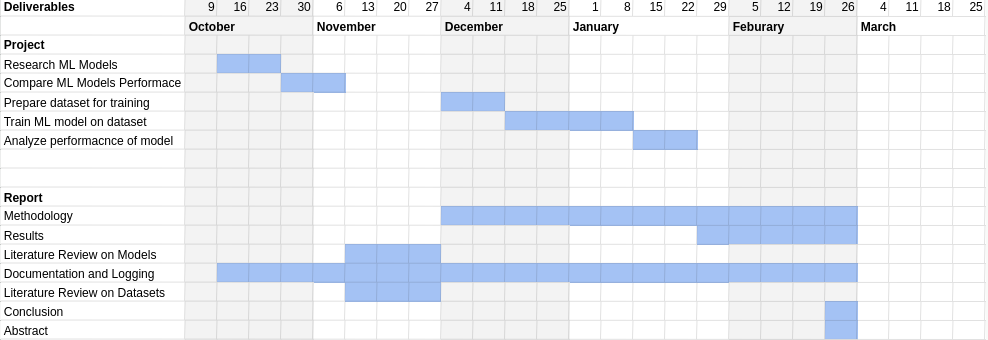
\includegraphics[width=\textwidth]{gantt_2}
\centering
\end{figure}


\subsection{Deliverables}

\begin{enumerate}
\item Project
\begin{itemize}
	\item Compare the performance of different \acrshort{ml} models.
	\item Produce an \acrshort{ml} model which can accurately predict preictal periods on EEG data.
	\item Organized data, including raw data and the preprocessed data, including the relevant literature.
\end{itemize}

\item Report
\begin{itemize}
    \item My methodology, the results, and a conclusion.
    \item Logs documenting activities, tasks, and changes throughout the project.
    \item A literature review of the subject area, including a review on the different datasets.
\end{itemize}

\end{enumerate}





\pagebreak

\printglossary[type=\acronymtype]
\printglossary

\pagebreak

\bibliographystyle{agsm}
\bibliography{references}

\end{document}